\hypertarget{introduction}{%
\section{Introduction}\label{introduction}}

\hypertarget{several-questions-under-one-name}{%
\subsection{Several questions under one
name}\label{several-questions-under-one-name}}

Observationally, dark energy enters cosmology as one fitted number,
\(\Omega_\Lambda \approx 0.7\) \citep{Riess1998, Perlmutter1999}. Around
that number sits a cluster of separate puzzles \citep{Abdalla2022}:

\begin{enumerate}
\def\labelenumi{\arabic{enumi}.}
\tightlist
\item
  the \textbf{cosmological-constant problem}: naive
  quantum-field-theoretic estimates of the vacuum energy exceed the
  observed value by up to about 120 orders of magnitude
  \citep{Weinberg1989, Martin2012};
\item
  the \textbf{Hubble tension}: early- and late-universe routes to
  \(H_0\) disagree at the several-\(\sigma\) level
  \citep{DiValentino2021};
\item
  \textbf{dataset inconsistencies}: supernova and BAO distances need not
  agree, and comparing standard candles with standard rulers gives a
  distance-duality consistency test \citep{BassettKunz2004};
\item
  \textbf{phantom crossing}: some joint fits of DESI DR2 with CMB and
  supernova data favor evolving equation-of-state histories that cross
  \(w=-1\) \citep{DESI2025DR2}, whereas a canonical, minimally coupled
  scalar field with positive energy density cannot cross, and scalar
  theories whose Lagrangian depends only on the field and its first
  derivatives cannot cross stably under regularity assumptions
  \citep{Caldwell2002, Vikman2005}, although some higher-derivative
  theories can \citep{Deffayet2010};
\item
  the \textbf{growth or \(S_8\) tension}: some low-redshift structure
  probes sit mildly below CMB-based expectations \citep{Heymans2021};
\item
  the \textbf{coincidence problem}: why the dark-energy and matter
  densities are comparable now \citep{Velten2014};
\item
  \textbf{interacting dark-sector models} and
\item
  \textbf{modified-gravity models}, both of which remain hard to
  separate from a cosmological constant on current data
  \citep{Clifton2012, Joyce2016};
\item
  the \textbf{anthropic question}: whether selection arguments should
  replace a derivation \citep{Weinberg1987}.
\end{enumerate}

These items are usually treated as one problem, to be solved by deriving
the value of \(\Lambda\) or predicting \(w(z)\) \citep{Copeland2006}.
They are in fact different kinds of question. Some ask what \emph{kind}
of term the constant is. One asks what fixes its \emph{value}. Some ask
which values are compatible with a universe that forms structure. One
asks whether our epoch is \emph{typical}. And several are questions
about the \emph{data}: which fits are preferred, and whether different
probes agree.

\hypertarget{approach}{%
\subsection{Approach}\label{approach}}

This paper treats these questions separately, using the closure calculus
of the Six Birds program
\citep{TsiokosSixBirds2026, TsiokosFoundations2026} as a common
vocabulary. In that calculus a theory is a \emph{closure package}: a
coarse description, a rule for filling in what the description leaves
out, and audits that test the result (Section 2). Two of its notions do
most of the work here. A \textbf{budget} with its \textbf{shadow price}
describes a global constraint and the multiplier that enforces it. A
\textbf{readout} is what a description records; asking whether one
readout determines a quantity is a precise question with a yes-or-no
answer.

For the questions studied here we specify finite-dimensional models or
data audits, state exactly what they contain, and ask what they
determine. The answers take three forms: theorems about the model (most
of them kernel-checked in Lean 4), computations on the model with
controls that could have failed, and pre-registered audits of public
data. We call the resulting separation of determined from undetermined
parts a \emph{demarcation}. It is always relative to a stated model and
a stated readout.

\hypertarget{results-in-brief}{%
\subsection{Results in brief}\label{results-in-brief}}

\begin{enumerate}
\def\labelenumi{\arabic{enumi}.}
\tightlist
\item
  \textbf{The constant slot as a price (Section 4).} If a convex closure
  problem attains its optimum and its optimal value is finite near the
  budget level and strictly improves when the budget is relaxed, the
  budget binds and carries a positive scalar price, with full Lagrangian
  optimality. In an allocation model with heterogeneous patches, every
  positive allocation sees the same price; for an originally binding
  budget, a common linear utility term \(s\sum_ix_i\) leaves the
  optimizer unchanged and shifts the price from \(p\) to \(p+s\), as
  long as \(p+s\ge0\); and the price is zero when the budget is slack.
\item
  \textbf{A record window (Section 5).} In a toy universe with linear
  structure growth, a declared collapse threshold and erasure of records
  at turnaround, at least ten of twelve sampled patch populations retain
  records of both tag values through the horizon exactly when
  \(-1/8000<\lambda\le\lambda_+\), with \(3<\lambda_+<3.4\). The lower
  edge is set by the declared horizon; if records need only form
  eventually and then persist forever, the window of this gate becomes
  \([0,u_\infty)\) with \(3<u_\infty<3.4\).
\item
  \textbf{What the readouts determine (Section 6).} In a self-consistent
  lattice model whose background offset is the analog of the constant
  term, the background does change the dynamics, but all eighteen
  sampled offsets converge. Fifteen pass a fixed sixty-update
  convergence test. Neither that test nor the existence of a limit
  recovers the offset. Adding a global density ledger makes the absolute
  background a gauge coordinate: it cannot be recovered from the
  invariant record, no selector that depends only on that record can
  follow a common shift, and no translation-invariant probability
  distribution over it exists.
\item
  \textbf{Typicality needs a prior (Section 7).} Five declared priors
  over the record window give different distributions of the coincidence
  ratio \(R=|\lambda|/\rho_m\) at the first record; on the sampled grid
  none meets the declared criterion of putting at least 80\% of its mass
  within one decade of the largest sampled ratio with a central 90\%
  interval at most 1.5 decades wide. A smooth, positive prior can put
  almost all its mass on arbitrarily small ratios, so regularity near
  \(\lambda=0\) cannot by itself settle the coincidence.
\item
  \textbf{Audits of real data (Section 8).} On DESI DR2, Pantheon+ and
  compressed Planck data, a rewrite family \(A(1+z)^m\) has a
  constant-compatible shape; the best-fit \(w_0w_a\) history crosses
  \(w=-1\) at \(z\approx0.439\), where its density is positive, smooth
  and maximal; and a staging audit on supernova and BAO subsets,
  calibrated on mock catalogues, flags structured dependence between the
  subsets, led by the high-redshift supernova split. A separate audit of
  growth data finds that no single surveyed probe covers both regimes
  that a decisive test would need.
\end{enumerate}

\hypertarget{what-contingent-modulus-means-here}{%
\subsection{What ``contingent modulus'' means
here}\label{what-contingent-modulus-means-here}}

A parameter is a \textbf{modulus} of a model, relative to a declared
readout, when that readout does not determine it: some two admissible
configurations with different values give the same readout. It is
\textbf{contingent} in the same relative sense: it must be supplied as
input or chosen by some additional rule. The title's claim is meant in
this sense and is established in two forms. In the original lattice
model, two convergence readouts fail to determine the background offset
(\Cref{thm:readout}). In the ledger-closed extension, no function of the
invariant record determines the absolute background, no selector
depending only on that record transforms correctly under a common shift,
and no translation-invariant probability distribution over the absolute
value exists (\Cref{thm:gauge}; the last statement is a standard
argument that is not mechanized).

Neither statement says that the physical cosmological constant is
intrinsically undetermined, that no richer readout could fix the model
parameter, or that no selection principle exists. They locate what a
selection principle would have to supply in the models studied.

\hypertarget{what-this-paper-does-not-claim}{%
\subsection{What this paper does not
claim}\label{what-this-paper-does-not-claim}}

The paper does not derive the value of \(\Lambda\) and does not refute a
fundamental cosmological constant. It does not identify the closure
price of Section 4 with the physical cosmological constant: that would
require a map from the model's budget to a gravitational field equation
with conserved stress-energy and the right dimensions and sign, which is
not constructed here. The toy universe of Section 5 is a declared model,
and its window is a property of its rules. The equation-of-state
analysis of Section 8 shows that one expansion history has two regular
descriptions; it does not decide whether physical dark energy is a
fluid, and it says nothing about ghosts. The one real-data detection
flags structured dependence between data subsets, consistent with a
known tension; it is not a new-physics signal and does not identify the
tension's source.

\begin{figure}[t]
\centering
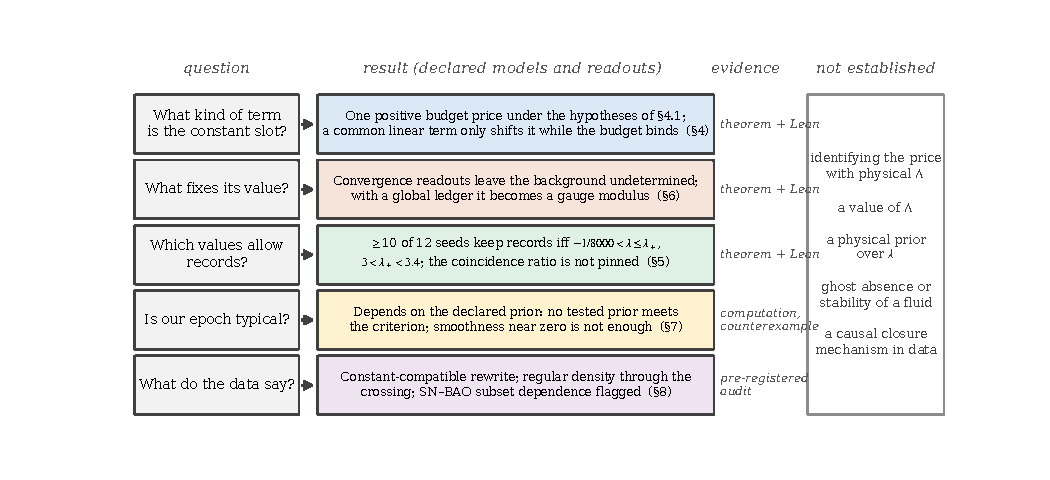
\includegraphics[width=\textwidth]{F1_overview.pdf}
\caption{\textbf{Overview.} Each dark-energy question is posed to a finite model or a data audit. The middle column
states what the paper establishes and the evidence type: a theorem (with Lean mechanization), a computation, or a
pre-registered audit. All results are relative to the declared models and readouts. The right column lists what is not
established.}
\label{fig:overview}
\end{figure}
